\documentclass[12pt]{article}
\usepackage[utf8]{inputenc}
\usepackage{geometry}
\geometry{a4paper, margin=1in}
\usepackage{tabularx}
\usepackage{enumitem}
\usepackage{booktabs}
\usepackage{xcolor}
\usepackage{titlesec}
\usepackage{hyperref}
\usepackage{caption}
\usepackage{float}

% 1. Added graphicx for your image files
% REMOVE "[demo]" once you actually have dfd.png and usecase.png in your folder!
\usepackage{graphicx} 

% 2. Kept all your original TikZ settings for the other diagrams
\usepackage{tikz}
\usetikzlibrary{arrows.meta,positioning,shapes.geometric,calc}

\definecolor{mNavy}{RGB}{30,58,138}
\definecolor{mDark}{RGB}{15,23,42}
\definecolor{mSlate}{RGB}{71,85,105}
\definecolor{mBlue}{RGB}{37,99,235}
\definecolor{mPurple}{RGB}{124,58,237}
\definecolor{mGreen}{RGB}{5,150,105}
\definecolor{mOrange}{RGB}{234,88,12}
\definecolor{mLight}{RGB}{248,250,252}

\hypersetup{colorlinks=true,linkcolor=mDark,urlcolor=mBlue}
\captionsetup{labelfont={bf,color=mDark},font=small,skip=8pt}
\titleformat{\section}{\normalfont\Large\bfseries\color{mDark}}{\thesection}{1em}{}[\titlerule]
\titleformat{\subsection}{\normalfont\large\bfseries\color{mDark}}{\thesubsection}{1em}{}

\tikzset{
flowbox/.style={rectangle,rounded corners=3pt,draw=mBlue,very thick,fill=mLight,minimum width=2.2cm,minimum height=1cm,align=center,text width=2.2cm,font=\small},
process/.style={ellipse,draw=mPurple,very thick,fill=mLight,minimum width=2.8cm,minimum height=1.1cm,align=center,font=\small},
datastore/.style={rectangle,draw=mOrange,very thick,fill=mLight,minimum width=2.8cm,minimum height=.9cm,align=center,font=\small},
entity/.style={rectangle,draw=mGreen,very thick,fill=mLight,minimum width=2.8cm,minimum height=.9cm,align=center,font=\small},
tier/.style={rectangle,rounded corners=4pt,draw=mBlue,very thick,fill=mLight,minimum width=4.8cm,minimum height=1.05cm,align=center},
arrow/.style={-{Latex[length=3mm]},thick,draw=mSlate}
}

\begin{document}

\begin{center}
\LARGE\textbf{Event Collision Detector: Predictive Launch-Window Intelligence}\\
\vspace{0.5em}
\Large\textbf{Project Proposal for UCS503P}\\
\vspace{0.5em}
\large Thapar Institute of Engineering and Technology
\end{center}

\vspace{1.5em}
\renewcommand{\arraystretch}{1.5}
\noindent
\begin{tabularx}{\textwidth}{|l|X|}
\hline
\textbf{Student Names} & Jaskaran Singh, Vaani Mehta, Parmeet Singh \\
\hline
\textbf{Roll Numbers} & 1024160033, 1024160123, 1024160021 \\
\hline
\textbf{Course} & Software Engineering (UCS503P) \\
\hline
\textbf{Submitted to} & Jeelani Asif \\
\hline
\end{tabularx}

\section{Higher-order goal}
The project aims to improve the success of high-stakes launches by reducing avoidable competition for audience attention, media coverage, and marketing visibility. The immediate engineering objective of the \textbf{Event Collision Detector} is to convert cross-industry event intelligence into an actionable scheduling decision by aggregating external events, evaluating a proposed launch window, generating an explainable collision-risk score, and recommending lower-risk alternatives.

\section{Time-to-value}
\begin{itemize}[leftmargin=0.7cm]
\item Deliver an initial single-industry event ingestion pipeline and heuristic collision score within the first iteration.
\item Prioritize fast feedback using existing event APIs and explainable rule-based scoring before introducing advanced predictive models.
\item Define first-iteration success as a complete date input $\rightarrow$ event retrieval $\rightarrow$ risk score $\rightarrow$ recommendation flow.
\end{itemize}

\section{Problem Statement}
Marketing and product teams often choose launch dates using internal schedules without sufficient visibility into the external event landscape.
\begin{itemize}[leftmargin=0.7cm]
\item \textbf{Blind-Spot Scheduling:} Internal calendars do not show competitor launches, industry conferences, or major public events.
\item \textbf{Diluted Audience Attention:} Overlapping events fragment media coverage and audience engagement.
\item \textbf{Sunk Marketing Spend:} A poorly timed launch can reduce the return on months of campaign preparation.
\item \textbf{No Systematic Alternative-Date Discovery:} Teams lack a structured way to identify nearby low-risk windows.
\end{itemize}

\section{Proposed Solution}
\subsection{Overview}
Build a web-based \textbf{Event Collision Detector} with the following components:
\begin{itemize}[leftmargin=0.7cm]
\item \textbf{Cross-Industry Event Radar:} Aggregates external events from APIs, conference schedules, and selected public sources into an indexed event catalog (\texttt{D2: Event Index}).
\item \textbf{Real-Time Collision Scoring:} Produces a High / Medium / Low risk score for a proposed date by searching nearby dates ($\pm 7$ days).
\item \textbf{Optimal Launch Recommendations:} Searches surrounding dates and returns lower-risk alternatives.
\item \textbf{Interactive Risk Dashboard:} Displays the risk score, conflicting events, and explanations.
\item \textbf{Calendar Syncing \& Source Management:} Allows users to sync finalized dates to Google/Outlook calendars and enables administrators to manage industry configurations and users.
\end{itemize}

\subsection{Core workflow}
\begin{enumerate}[leftmargin=0.7cm]
\item \textbf{Ingest \& Normalize:} Ingestion jobs continuously normalize raw event data into \texttt{D2: Event Index (Elasticsearch)} based on admin industry rules.
\item \textbf{Process Submission:} User submits launch date details; validated parameters and user session records are logged to \texttt{D1: User Store (PostgreSQL)}.
\item \textbf{Retrieve Events:} System queries \texttt{D2} for competing events occurring within $\pm 7$ days of the target date.
\item \textbf{Compute Risk \& Recommendations:} Scoring engine computes collision risk, identifies primary drivers, and identifies low-risk alternative launch windows.
\item \textbf{Render Dashboard:} Interactive dashboard renders collision risk scores, event breakdowns, and recommended date cards.
\item \textbf{Sync Confirmed Date:} User selects a final date, updating \texttt{D1} and pushing an OAuth event payload to external calendar platforms (Google/Outlook).
\end{enumerate}

% Restored Original Core Workflow TikZ
\begin{figure}[H]
\centering
\resizebox{0.98\textwidth}{!}{
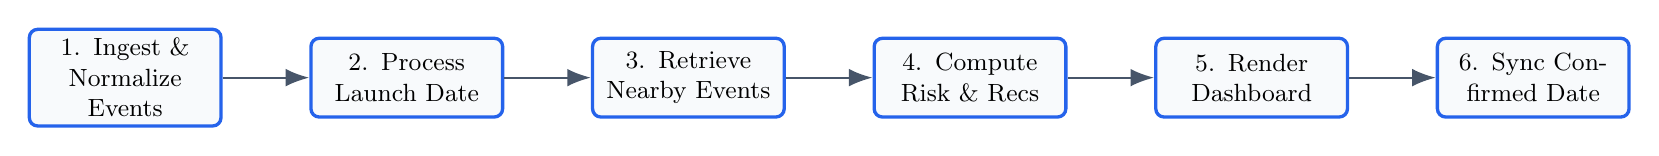
\begin{tikzpicture}[node distance=1.1cm]
\node[flowbox] (a) {1. Ingest \& Normalize Events};
\node[flowbox,right=of a] (b) {2. Process Launch Date};
\node[flowbox,right=of b] (c) {3. Retrieve Nearby Events};
\node[flowbox,right=of c] (d) {4. Compute Risk \& Recs};
\node[flowbox,right=of d] (e) {5. Render Dashboard};
\node[flowbox,right=of e] (f) {6. Sync Confirmed Date};
\draw[arrow] (a)--(b); \draw[arrow] (b)--(c); \draw[arrow] (c)--(d); \draw[arrow] (d)--(e); \draw[arrow] (e)--(f);
\end{tikzpicture}}
\caption{Event Collision Detector Core Workflow Execution Pipeline (Aligned with Level 1 DFD)}
\end{figure}

\subsection{Operational constraints for an educational setting}
\begin{itemize}[leftmargin=0.7cm]
\item Limit initial event coverage to selected industries such as Technology and Entertainment.
\item Prefer existing APIs and structured public feeds over large-scale scraping infrastructure.
\item Use heuristic, explainable scoring so that each risk score can be traced to specific events.
\item Keep the system deployable on standard cloud infrastructure or containerized local environments.
\end{itemize}

\section{System Analysis \& Behavioral Diagrams}

\subsection{Level 1 Data Flow Diagram (DFD)}
The Level 1 DFD models the flow of data across the system entities, processes, and persistent data stores.

\begin{figure}[H]
\centering
% This is where your external DFD image goes

\includegraphics[width=0.95\textwidth, height=8cm]{dfd.png}
\caption{Level 1 Data Flow Diagram (DFD) for Event Collision Detector}
\end{figure}

\subsection{Use Case Diagram}
The Use Case Diagram defines the interactions between key system actors and the primary functional features.

\begin{figure}[H]
\centering
% This is where your external Use Case image goes

\includegraphics[width=0.95\textwidth, height=10cm]{usecase.png}
\caption{System Use Case Diagram with Actors and Boundary Constraints}
\end{figure}

\section{Solution Approach}
This project focuses on software engineering, event ingestion, low-latency retrieval, explainable scoring, and a responsive dashboard rather than novel machine-learning research.

\subsection{Collision analysis logic}
\begin{itemize}[leftmargin=0.7cm]
\item \textbf{Temporal Proximity:} Events closer to the proposed date ($\pm 7$ day window) receive greater weight.
\item \textbf{Industry Relevance:} Same-industry or related events contribute more strongly to risk.
\item \textbf{Audience Overlap:} Similar target-audience tags increase attention conflict.
\item \textbf{Event Magnitude:} Larger events receive greater importance.
\item \textbf{Media Friction:} Events competing for similar channels or press attention increase the score.
\end{itemize}

% Restored Original Collision Logic TikZ
\begin{figure}[H]
\centering
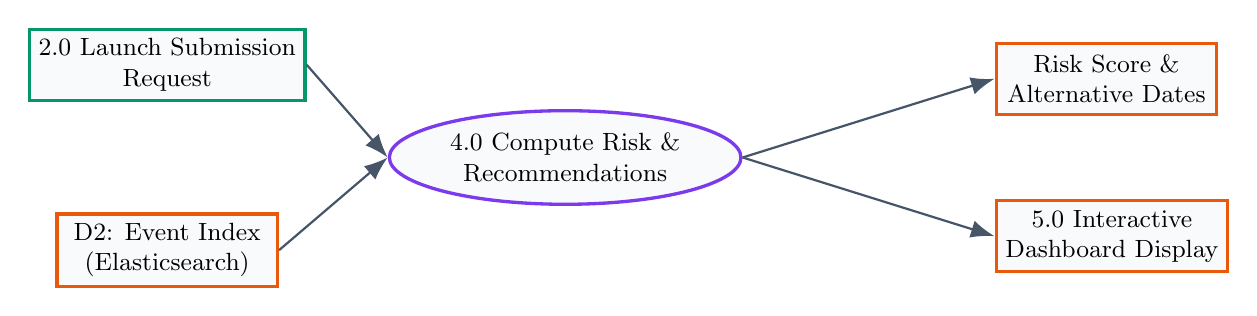
\begin{tikzpicture}[node distance=1.4cm and 2.0cm]
\node[entity] (planned) {2.0 Launch Submission\\Request};
\node[datastore,below=of planned] (external) {D2: Event Index\\(Elasticsearch)};
\node[process,right=2.8cm of $(planned)!0.5!(external)$] (engine) {4.0 Compute Risk \&\\Recommendations};
\node[datastore,right=3.2cm of engine,yshift=1.0cm] (risk) {Risk Score \&\\Alternative Dates};
\node[datastore,right=3.2cm of engine,yshift=-1.0cm] (conflicts) {5.0 Interactive\\Dashboard Display};
\draw[arrow] (planned.east)--(engine.west);
\draw[arrow] (external.east)--(engine.west);
\draw[arrow] (engine.east)--(risk.west);
\draw[arrow] (engine.east)--(conflicts.west);
\end{tikzpicture}
\caption{Collision Analysis and Explainable Risk-Scoring Logic}
\end{figure}

\subsection{System architecture}
A layered architecture separates user interaction, application logic, scoring, ingestion, and persistent storage.
\begin{itemize}[leftmargin=0.7cm]
\item \textbf{Frontend Dashboard:} React.js + Tailwind CSS for rendering the interactive dashboard and calendar sync actions.
\item \textbf{API Layer:} FastAPI backend handling submission processing, date retrieval, and OAuth calendar synchronization.
\item \textbf{Collision Scoring Service:} Python analysis service executing proximity and audience collision heuristics.
\item \textbf{Data Ingestion Layer:} Ingestion service that retrieves raw data from External Event APIs and normalizes records into Elasticsearch.
\item \textbf{Storage Layer:} Dual-store database setup featuring \texttt{D1: User Store (PostgreSQL)} for user/session records and confirmed events, and \texttt{D2: Event Index (Elasticsearch)} for fast $\pm 7$ day date-range queries.
\end{itemize}

% Restored Original Architecture TikZ
\begin{figure}[H]
\centering
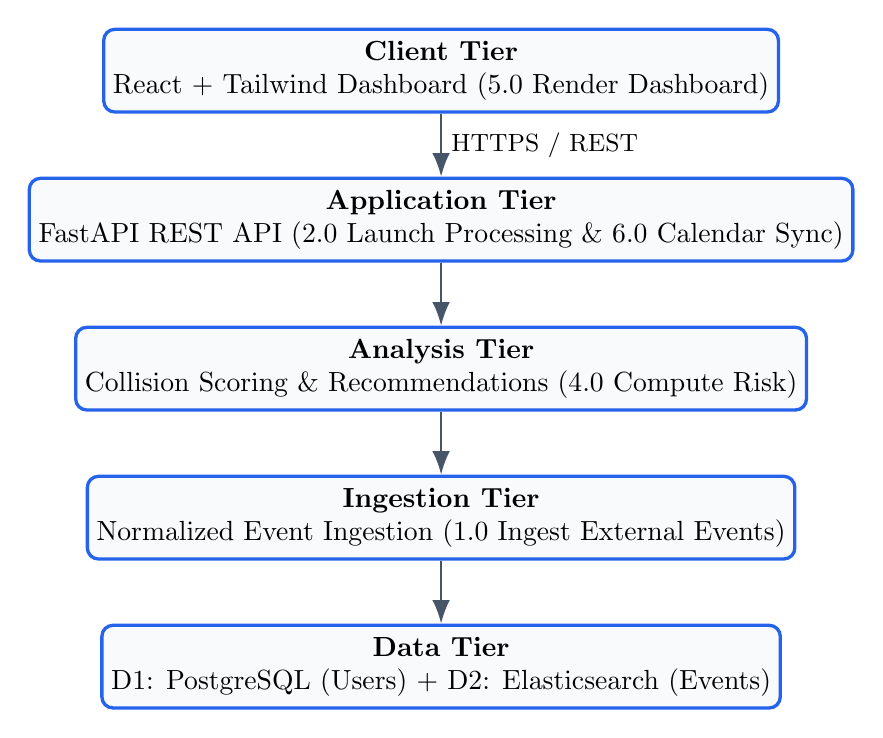
\begin{tikzpicture}[node distance=0.8cm]
\node[tier] (client) {\textbf{Client Tier}\\React + Tailwind Dashboard (5.0 Render Dashboard)};
\node[tier,below=of client] (api) {\textbf{Application Tier}\\FastAPI REST API (2.0 Launch Processing \& 6.0 Calendar Sync)};
\node[tier,below=of api] (logic) {\textbf{Analysis Tier}\\Collision Scoring \& Recommendations (4.0 Compute Risk)};
\node[tier,below=of logic] (ingest) {\textbf{Ingestion Tier}\\Normalized Event Ingestion (1.0 Ingest External Events)};
\node[tier,below=of ingest] (data) {\textbf{Data Tier}\\D1: PostgreSQL (Users) + D2: Elasticsearch (Events)};
\draw[arrow] (client)--node[right]{\small HTTPS / REST}(api);
\draw[arrow] (api)--(logic); \draw[arrow] (logic)--(ingest); \draw[arrow] (ingest)--(data);
\end{tikzpicture}
\caption{Event Collision Detector Layered Web Architecture}
\end{figure}

\subsection{CI/CD and fast delivery enabler}
CI/CD pipelines will run unit tests for scoring and normalization logic, verify frontend-backend API contracts, validate builds, and publish project documentation through GitHub Actions.

\section{Evaluation Criterion}
\subsection{Primary evaluation metric}
\textbf{Collision Score Latency (CSL):} Time from proposed-event submission to returned risk score and recommendation set.
\begin{itemize}[leftmargin=0.7cm]
\item \textbf{Target:} Median CSL $\leq 500$ ms against an indexed Elasticsearch event dataset (\texttt{D2}).
\item \textbf{Measurement:} Backend request timing recorded for each scoring request.
\end{itemize}

\subsection{Secondary evaluation metrics}
\begin{itemize}[leftmargin=0.7cm]
\item \textbf{Scoring Agreement:} At least 80\% agreement with manual assessment on a labeled validation set.
\item \textbf{Ingestion Freshness:} Newly published API events reflected in \texttt{D2} within 24 hours of the ingestion cycle.
\item \textbf{Recommendation Quality:} At least 90\% of recommended dates should have a lower score than the original date.
\item \textbf{Dashboard Responsiveness:} Risk details and recommendations render on the interactive dashboard within one second after the API response.
\end{itemize}

\subsection{Pilot validation plan}
Test historical launch dates against manually researched competing events and conduct a small usability trial with students role-playing marketing or product managers.

\section{Scalability}
\begin{enumerate}[leftmargin=0.7cm]
\item \textbf{Scalable theoretically:} Separate ingestion (\texttt{1.0}) from scoring (\texttt{4.0}), cache repeated date windows in Elasticsearch (\texttt{D2}), and introduce query optimization as event volume grows.
\item \textbf{Operationally deployable practically:} Containerize frontend and backend, add industries through new source configurations, and run initially on PostgreSQL (\texttt{D1}) and Elasticsearch (\texttt{D2}).
\end{enumerate}

\section{Engine availability heuristic}
\begin{itemize}[leftmargin=0.7cm]
\item \textbf{React + Tailwind CSS:} Frontend dashboard and interactive rendering.
\item \textbf{FastAPI:} Python backend for event, scoring, and calendar sync endpoints.
\item \textbf{PostgreSQL (\texttt{D1}):} Storage for user accounts, session records, and updated finalized events.
\item \textbf{Elasticsearch (\texttt{D2}):} Index for normalized external events and low-latency date-range filtering.
\item \textbf{Pandas / Scikit-learn:} Data preprocessing and scoring utilities.
\item \textbf{External Event APIs / OAuth:} Ingestion sources (Eventbrite/PredictHQ) and calendar push platforms (Google/Outlook).
\item \textbf{GitHub Actions:} Automated testing and CI/CD.
\end{itemize}

\section{Project scope and deliverables}
\subsection{Initial deliverable}
\begin{itemize}[leftmargin=0.7cm]
\item Basic React dashboard for event submission and rendering.
\item One external event source integrated into the ingestion pipeline (\texttt{1.0}).
\item Working FastAPI endpoint returning High / Medium / Low collision risk (\texttt{4.0}).
\item Risk breakdown showing the events responsible for the score.
\item PostgreSQL (\texttt{D1}) and Elasticsearch (\texttt{D2}) persistence setup.
\item Automated CI pipeline for linting, testing, and build validation.
\end{itemize}

\subsection{Subsequent deliverables}
\begin{itemize}[leftmargin=0.7cm]
\item Additional event sources and industry coverage.
\item Alternative-date recommendation engine.
\item OAuth calendar synchronization for Google and Outlook platforms (\texttt{6.0}).
\item Administrator interface for user and event database management.
\end{itemize}

\section{Risks and mitigations}
\begin{itemize}[leftmargin=0.7cm]
\item \textbf{API Rate Limits / Data Gaps:} Cache retrieved events in \texttt{D2} and reduce confidence when source data is incomplete.
\item \textbf{Scoring Heuristic Inaccuracy:} Validate weights against manually labeled historical examples.
\item \textbf{Cold-Start Coverage:} Seed the Elasticsearch index with an initial historical batch.
\item \textbf{Inconsistent Event Metadata:} Normalize incoming events into a common schema during Process \texttt{1.0} before scoring.
\item \textbf{Over-Engineering:} Keep the first version limited to one or two industries and an explainable scoring function.
\end{itemize}

\section{Summary}
The \textbf{Event Collision Detector} is a deployable scheduling-intelligence platform that helps teams avoid launching into crowded attention windows. It combines external event aggregation, explainable collision scoring, and alternative-date recommendations in a single web dashboard. The project emphasizes rapid time-to-value, measurable evaluation criteria, modular architecture, mature tooling, and a clear path from prototype to scalable product.

\end{document}
